\documentclass[11pt]{article}

\usepackage[margin=1in]{geometry}
\usepackage[T1]{fontenc}
\usepackage[utf8]{inputenc}
\usepackage{amsmath,amssymb}
\usepackage{booktabs}
\usepackage{array}
\usepackage{tabularx}
\usepackage{multirow}
\usepackage{longtable}
\usepackage{graphicx}
\usepackage{xcolor}
\usepackage{float}
\usepackage{enumitem}
\usepackage{hyperref}
\usepackage{titlesec}
\usepackage{caption}
\usepackage{fancyhdr}
\usepackage{listings}
\usepackage{url}

\pagestyle{fancy}
\fancyhf{}
\fancyhead[L]{EcoExplain-VLM}
\fancyhead[R]{\thepage}
\renewcommand{\headrulewidth}{0.4pt}
\setlength{\headheight}{14pt}

\title{
\textbf{EcoExplain-VLM:}\\
An Explainable Vision-Language Framework for Forest Disturbance Analysis\\
Using Multimodal Geospatial Data
}
\author{
\textit{Research Project Report}\\[0.5em]
Author: [Your Name]\\
Institution: [Your Institution]\\
Course / Research Project: [Course / Independent Study]\\
Date: \today\\
Study Region: Kanha Tiger Reserve
}
\date{}

\newcommand{\status}[1]{\textbf{#1}}
\newcommand{\verify}[1]{\textit{Note: #1}}

\setlength{\parindent}{0pt}
\setlength{\parskip}{0.5em}

\begin{document}

\maketitle

\begin{abstract}
This report presents EcoExplain-VLM, an Independent Study benchmark and evaluation pipeline for forest vegetation change at Kanha Tiger Reserve, Madhya Pradesh, using matched dry-season windows (January--February 2022 vs.\ 2023). For each of \textbf{366} forest patches ($\sim$640\,m scale), five geospatial streams were assembled---Sentinel-2 optical imagery and vegetation indices, Sentinel-1 SAR, CHIRPS rainfall, ERA5-Land temperature and soil-moisture anomalies, and NASADEM terrain---and encoded as paired RGB chips plus structured evidence text in \texttt{dataset.jsonl}, with stratified train/dev/test splits (256/55/55, seed 42).

Four open vision--language models (0.5--3B parameters) were evaluated under \textbf{Condition~C} (images plus multimodal evidence) on a shared held-out test set ($n=55$). \textbf{Qwen2-VL-2B} achieved the strongest zero-shot accuracy (\textbf{56.4\,\%}), ahead of PaliGemma (36.4\,\%) and LLaVA-Interleave / BLIP-2 (32.7\,\% each). \textbf{LoRA fine-tuning} on Ada further raised Qwen test accuracy to \textbf{67.3\,\%} (smoke configuration: 16 training patches, one epoch). These classification outcomes form the primary quantitative benchmark reported here.

The study then focuses on \textbf{explanation quality}: models were prompted for a class decision with a justification, and outputs were scored automatically for evidence-consistent claims (\texttt{scripts/score\_explanations.py}). With a free-form prompt, PaliGemma and BLIP-2 produced almost no checkable claims and LLaVA generated fluent but repetitive text (56.7\,\% of checkable claims correct). A structured cite-only prompt, run on all 55 test patches on a MacBook Air (Apple MPS) in October 2026, raised claim correctness to \textbf{75.8\,\%} for Qwen2-VL-2B and \textbf{71.1\,\%} for LLaVA-Interleave-0.5B, with claims agreeing with the stated class in 100\,\% and 90.7\,\% of explanations. Under this prompt the class follows a stated NDVI rule, and justifications mostly restate supplied facts. Free-form explanations from small open VLMs are therefore unreliable, while constraining them to cite verified facts makes them consistent with the evidence.

The report documents data engineering, the evaluation protocol, results, limitations, and directions for spatial validation, human faithfulness rating, and domain-aligned multimodal encoders. All headline metrics are traceable to JSON outputs under \texttt{results/}.
\end{abstract}

\vspace{0.5em}
\noindent\textbf{Keywords:} vision--language models; forest vegetation change; multimodal remote sensing; Kanha Tiger Reserve; explainable artificial intelligence; LoRA fine-tuning; evidence-grounded explanations

\tableofcontents
\listoftables
\listoffigures

\section{Introduction}

\subsection{Problem Statement}
Forest disturbance monitoring is a critical task for biodiversity conservation, ecosystem resilience, climate assessment, and sustainable land management. Disturbance events can include deforestation, degradation, vegetation stress, fire damage, and other forms of structural or ecological change. Monitoring these changes requires repeated observations over space and time, particularly in protected areas where disturbances may be subtle, patch-based, or difficult to distinguish using a single sensor modality.

Remote sensing provides a scalable way to observe these changes, but the problem is not only detection; it is also explanation. A system that can identify change is useful, but a system that can explain why the change is occurring, what evidence supports the classification, and which remote sensing signals contributed to the decision is far more useful to practitioners, ecologists, and researchers.

\subsection{Motivation}
The motivation behind EcoExplain-VLM is to combine geospatial evidence with multimodal reasoning to generate disturbance classifications and explanatory outputs that are understandable to humans. Optical imagery captures vegetation reflectance and spectral response. SAR captures structural and moisture-related information independent of sunlight conditions. Thermal and environmental variables provide context related to climate anomalies, soil conditions, or terrain. Vision-language models provide a way to map these multimodal inputs into structured textual reasoning and answer generation.

The project therefore aims to move beyond a pure predictive classifier toward a framework that is both evidence-aware and explainable. This is especially relevant in forest monitoring, where model predictions may be accepted more readily when grounded in observable patterns such as vegetation loss, changes in moisture, or disturbed canopy structure.

\subsection{Research Objective}
The main objective was to construct and evaluate an explainable multimodal VLM-based framework for forest disturbance analysis using geospatial evidence from multiple sources, with emphasis on \textbf{Condition~C classification} and subsequent \textbf{analysis of explanation quality}.

\subsection{Secondary Objectives}
The secondary objectives include:
\begin{itemize}
    \item building a geospatial dataset of before/after forest patches;
    \item integrating optical, SAR, climate, and terrain features;
    \item generating disturbance-oriented evidence cards for each patch;
    \item evaluating multiple VLM backbones in a controlled benchmark;
    \item testing fine-tuned performance on a classification task;
    \item assessing whether the model produces interpretable, evidence-grounded explanations.
\end{itemize}

\subsection{Research Questions}
The project is guided by several research questions:
\begin{enumerate}
    \item Can multimodal remote sensing inputs support forest disturbance classification?
    \item Are optical and SAR features complementary for detecting ecological change?
    \item Can a VLM integrate image evidence and structured geospatial signals into a stable classification output?
    \item Can the model provide explanations that are grounded in measurable evidence rather than generic narrative?
    \item Does a fine-tuned VLM outperform zero-shot baselines on this task?
\end{enumerate}

\subsection{Hypotheses}
The project implicitly tests the following hypotheses:
\begin{itemize}
    \item Multimodal geospatial evidence is more informative than a single sensor alone.
    \item Vegetation indices and disturbance masks capture informative change signals.
    \item A VLM can interpret these signals when presented as structured image and text evidence.
    \item Fine-tuning improves performance beyond baseline zero-shot evaluation.
\end{itemize}

\subsection{Expected Contribution and Novelty}
The expected contribution is a research-oriented multimodal pipeline that unifies remote sensing, geospatial feature reasoning, and VLM-based classification/explanation. The novelty lies in the combination of:
\begin{itemize}
    \item optical + SAR + climate + terrain data,
    \item disturbance-region extraction using spectral change masks,
    \item prompt-based VLM classification,
    \item and explanation generation using evidence cards.
\end{itemize}

\subsection{Outcomes at a Glance}
The project delivered a reproducible Kanha benchmark, a four-model Condition~C classification study with \textbf{Qwen2-VL-2B at 56.4\,\%} zero-shot and \textbf{67.3\,\%} after LoRA fine-tuning on the held-out test set, and an explanation-evaluation track: free-form explanations were weakly grounded, while a structured cite-only prompt raised claim correctness to 75.8\,\% (Qwen) and 71.1\,\% (LLaVA) on the full test set. Classification performance is reported under the project's Condition~C protocol, whose evidence card includes the pipeline's summary line; explanation analysis is the main interpretive contribution.

\section{Study Area and Temporal Design}

\subsection{Study Region}
The project uses a study region in \textbf{Kanha Tiger Reserve}, which is a major forested ecosystem in central India. The area is ecologically important due to its biodiversity, tiger habitat, and forest cover structure. A protected area such as Kanha is appropriate for disturbance analysis because:
\begin{itemize}
    \item forest cover is ecologically significant;
    \item subtle vegetation change matters for conservation monitoring;
    \item repeated observations allow temporal comparison;
    \item remote sensing can reveal degradation and fragmentation patterns.
\end{itemize}

The project defines a region of interest (ROI) and patch-based sampling around the selected area. The actual implementation is configured through project config files and the patch extraction logic.

\subsection{Temporal Experiment}
The project compares two dry-season periods:
\begin{itemize}
    \item \textbf{T0}: January--February 2022
    \item \textbf{T1}: January--February 2023
\end{itemize}

This temporal design is reasonable because:
\begin{itemize}
    \item both periods fall in the dry season;
    \item seasonal conditions are more comparable than comparing dissimilar phenological periods;
    \item vegetation change is more interpretable when excluding major seasonal confounds.
\end{itemize}

The code and project metadata indicate a matched dry-season comparison. However, the exact temporal comparability and ecological assumptions should be viewed as a practical pilot design rather than a full multi-year time-series analysis.

\subsection{Why These Dates Were Chosen}
The project selected T0 and T1 to compare forest state before and after a change period while keeping seasonal effects controlled as much as possible. This was likely done to reduce variability associated with monsoon-driven phenology and seasonal vegetation cycles.

\subsection{Study-Area Characteristics}
The actual project files indicate a geospatial ROI configuration and patch extraction process. The study area is not treated as a broad continental scene but as a set of local patches extracted from a defined AOI. This spatially localized design supports evidence-card generation and VLM evaluation.

\subsection{AOI and Patch Design}
The project uses a patch-based representation of the landscape, with each patch corresponding to a local region of interest that contains image and feature evidence for a given time pair. In the final implementation, the project operates on a patch discretization over a selected area, with patches identified by unique IDs.

% --- For a tighter submission draft: consider moving Sections ``Remote Sensing Foundations'' through ``Environmental and Terrain Variables'' to an appendix to reduce textbook material.

\section{Remote Sensing Foundations}

\subsection{What Is Remote Sensing?}
Remote sensing is the acquisition of information about a target without direct physical contact. In environmental monitoring, it usually refers to sensing the Earth from airborne or spaceborne platforms. The data are typically represented as raster grids, where each cell or pixel encodes a measured quantity such as reflected sunlight or microwave backscatter.

\subsection{Raster Data, Pixels, and Spatial Resolution}
A raster is a regular grid of values. Each grid cell is a pixel. In remote sensing, pixel size corresponds to ground sampling distance (GSD), which indicates the physical size of each cell on Earth.

If a sensor pixel is 10 m, then each pixel covers approximately $10 \times 10$ meters on the ground. If a patch is $64 \times 64$ pixels at 10 m resolution, then the physical area is approximately:
\[
64 \times 10\text{ m} = 640\text{ m}
\]
in each direction, producing a patch of around
\[
640 \times 640\text{ m}^2.
\]

This is an important design choice because it balances local ecological context with computational tractability.

\subsection{Spectral, Temporal, and Radiometric Resolution}
The project relies on spectral imagery and time-series comparison. The relevant concepts are:
\begin{itemize}
    \item \textbf{Spectral resolution}: the number and width of wavelength bands measured by a sensor.
    \item \textbf{Temporal resolution}: how often the sensor revisits a location.
    \item \textbf{Radiometric resolution}: the number of digital values available to represent signal intensity.
    \item \textbf{Reflectance}: the fraction of incoming radiation reflected by a surface.
    \item \textbf{Backscatter}: the fraction of radar signal returned to the sensor.
\end{itemize}

\subsection{Georeferencing and CRS}
Remote sensing data are georeferenced to a coordinate reference system (CRS), allowing pixels to be aligned spatially. Raster reprojection and resampling may be required when combining datasets from different sensors or when aligning data to a common grid.

\subsection{Sentinel-2 and MSI}
Sentinel-2 is part of the European Copernicus program and provides multispectral optical imagery. The sensor records reflectance in multiple bands from visible to shortwave infrared. The Multispectral Instrument (MSI) is the instrument onboard Sentinel-2.

The relevant bands used in project discussion are:
\begin{table}[H]
\centering
\renewcommand{\arraystretch}{1.2}
\begin{tabular}{p{1cm} p{1.7cm} p{2.4cm} p{5.6cm}}
\toprule
\textbf{Band} & \textbf{Wavelength} & \textbf{Resolution} & \textbf{Meaning} \\
\midrule
B1 & 443 nm & 60 m & Aerosol / atmospheric correction \\
B2 & 490 nm & 10 m & Blue \\
B3 & 560 nm & 10 m & Green \\
B4 & 665 nm & 10 m & Red \\
B5 & 705 nm & 20 m & Red edge \\
B6 & 740 nm & 20 m & Red edge \\
B7 & 783 nm & 20 m & Red edge \\
B8 & 842 nm & 10 m & Near infrared (NIR) \\
B8A & 865 nm & 20 m & Narrow NIR \\
B9 & 940 nm & 60 m & Water vapor \\
B11 & 1610 nm & 20 m & SWIR \\
B12 & 2190 nm & 20 m & SWIR \\
\bottomrule
\end{tabular}
\caption{Relevant Sentinel-2 bands and their role in vegetation analysis.}
\end{table}

These bands matter because vegetation reflects differently in red and NIR, which allows estimation of vegetation vigor and change.

\subsection{Vegetation Indices Used}
The project explicitly uses vegetation and disturbance indices. These are derived from reflective optical measurements.

\subsubsection{NDVI}
Normalized Difference Vegetation Index:
\[
NDVI = \frac{NIR - Red}{NIR + Red}
\]
Meaning:
\begin{itemize}
    \item high values indicate healthy, photosynthetically active vegetation;
    \item low values indicate bare soil, senescence, or disturbance.
\end{itemize}

\subsubsection{EVI}
Enhanced Vegetation Index:
\[
EVI = G \cdot \frac{NIR - Red}{NIR + C_1 Red - C_2 Blue + L}
\]
where \(G\) is gain, \(C_1\), \(C_2\), and \(L\) are calibration constants. EVI can be more robust under atmospheric effects and high biomass conditions.

\subsubsection{NDMI}
Normalized Difference Moisture Index:
\[
NDMI = \frac{NIR - SWIR}{NIR + SWIR}
\]
This is sensitive to plant water content and moisture state.

\subsubsection{NBR}
Normalized Burn Ratio:
\[
NBR = \frac{NIR - SWIR}{NIR + SWIR}
\]
This index is commonly used to detect fire and burn severity. It is especially relevant where disturbance is associated with vegetation loss or fire damage.

\subsubsection{How the Code Uses These Indices}
The actual project files indicate that NDVI, EVI, NDMI, and NBR are calculated or loaded as part of the geospatial processing stack. The downstream disturbance logic uses delta masks and bounding boxes to identify local change. The exact implementation is in the geospatial and DIP utilities.

\status{Verified:} the project includes these indices in the dataset pipeline.\\
\status{Verified as final input:} the model receives structured evidence cards and image inputs derived from the processed scene data.\\
\status{Caveat:} not every index must be used by the final VLM in the same way; implementation must be confirmed at the specific code path.

\section{Synthetic Aperture Radar (SAR) Background}

\subsection{What Is SAR?}
Synthetic Aperture Radar is an active sensing technology that emits microwave signals and records the backscattered energy from the Earth’s surface. Unlike optical sensors, SAR does not depend on sunlight and can operate in cloudy conditions.

\subsection{Why SAR Matters}
SAR is extremely useful in forest monitoring because it responds to:
\begin{itemize}
    \item vegetation structure;
    \item canopy roughness;
    \item soil moisture;
    \item moisture content in biomass;
    \item surface roughness and scattering geometry.
\end{itemize}

This is especially valuable when optical data are affected by clouds, haze, or seasonal vegetation variation.

\subsection{Active vs Passive Sensing}
Optical sensors are passive. They measure reflected sunlight. SAR is active: it emits its own microwave pulse and measures the returned signal. This gives it a different observational bias and complementary information content.

\subsection{Sentinel-1}
Sentinel-1 is the SAR mission in the Copernicus program. It provides C-band radar observations with useful temporal coverage, making it suitable for repeated disturbance monitoring.

The project’s implementation is based on sentinel-1 features and uses the relevant polarization channels:
\begin{itemize}
    \item \textbf{VV}: vertical transmit, vertical receive;
    \item \textbf{VH}: vertical transmit, horizontal receive.
\end{itemize}

\subsection{VV and VH in Practice}
VV and VH are helpful because they respond differently to:
\begin{itemize}
    \item vegetation volume scattering;
    \item canopy structure;
    \item surface roughness;
    \item moisture and trunk-ground interactions.
\end{itemize}

In forest settings, changes in canopy structure or vegetation density can produce measurable differences in the backscatter signal.

\subsection{Speckle}
Speckle is a form of multiplicative noise in SAR imagery caused by coherent microwave interference. It creates a grainy appearance and can obscure patterns. In practice, speckle is often reduced through filtering or multi-temporal aggregation. The project files indicate the use of SAR-derived features, but the exact speckle-handling strategy must be checked against the implementation.

\subsection{How SAR Helps in This Project}
The project uses SAR as one of the multimodal sources that can complement optical change detection. This is particularly relevant because forest disturbance may cause:
\begin{itemize}
    \item canopy loss;
    \item structural change in vegetation;
    \item changes in moisture or roughness.
\end{itemize}
These changes may not be visible in optical data alone or may be difficult to interpret under cloud or atmospheric conditions.

\section{Environmental and Terrain Variables}

\subsection{ERA5-Land}
ERA5-Land provides reanalysis variables at a spatial and temporal resolution suitable for environmental context. Variables may include anomalies in temperature, moisture, and surface conditions. The project uses ERA5-based features in its pipeline.

\subsection{DEM and Terrain}
The project also includes digital elevation model (DEM) and terrain features, which can help contextualize vegetation change and hydrological patterns. Terrain variables can be relevant for identifying areas that are more likely to experience moisture stress or slope-related disturbance patterns.

\subsection{Why Environmental Variables Matter}
Environmental variables are useful because disturbance is not purely visual. Vegetation stress can be associated with:
\begin{itemize}
    \item anomalous temperature,
    \item moisture deficits,
    \item terrain controls,
    \item and local environmental context.
\end{itemize}

These variables are not always directly visible in a single optical image, but they can help interpret change.

\section{Dataset and Project Structure}

\subsection{Repository Layout}
The project repository contains the following broad categories:
\begin{itemize}
    \item configuration files;
    \item data directories for raw, processed, splits, and outputs;
    \item scripts for export, build, validation, and evaluation;
    \item notebooks for analysis;
    \item source modules for geospatial processing and VLM evaluation;
    \item results files for benchmarks and comparisons.
\end{itemize}

\begin{table}[H]
\centering
\renewcommand{\arraystretch}{1.2}
\begin{tabular}{p{4cm} p{7cm}}
\toprule
\textbf{Folder / File} & \textbf{Purpose} \\
\midrule
configs/ & Study-area configuration and temporal settings \\
data/raw\_tiffs/ & Raw geotiffs from sensor sources \\
data/processed\_images/ & Derived images and patch-level renders \\
data/evidence\_masks/ & Disturbance masks and change masks \\
data/splits/ & Train, dev, and test split definitions \\
notebooks/ & Interactive pipeline steps and exploration \\
scripts/ & Export, validation, dataset building, and evaluation scripts \\
src/ & Source modules for geospatial processing, evaluation, and model logic \\
results/ & Benchmark outputs and comparison summaries \\
\bottomrule
\end{tabular}
\caption{High-level project structure.}
\end{table}

\section{Pipeline Overview}

The following pipeline is the most defensible representation of the actual project flow, based on the available code and generated outputs.

\[
\text{Raw geospatial data}
\to
\text{AOI and date filtering}
\to
\text{Preprocessing}
\to
\text{Index and feature generation}
\to
\text{Patch extraction}
\to
\text{Evidence-card assembly}
\to
\text{VLM prompting and classification}
\to
\text{Explanation generation}
\to
\text{Evaluation}
\]

\begin{figure}[H]
\centering
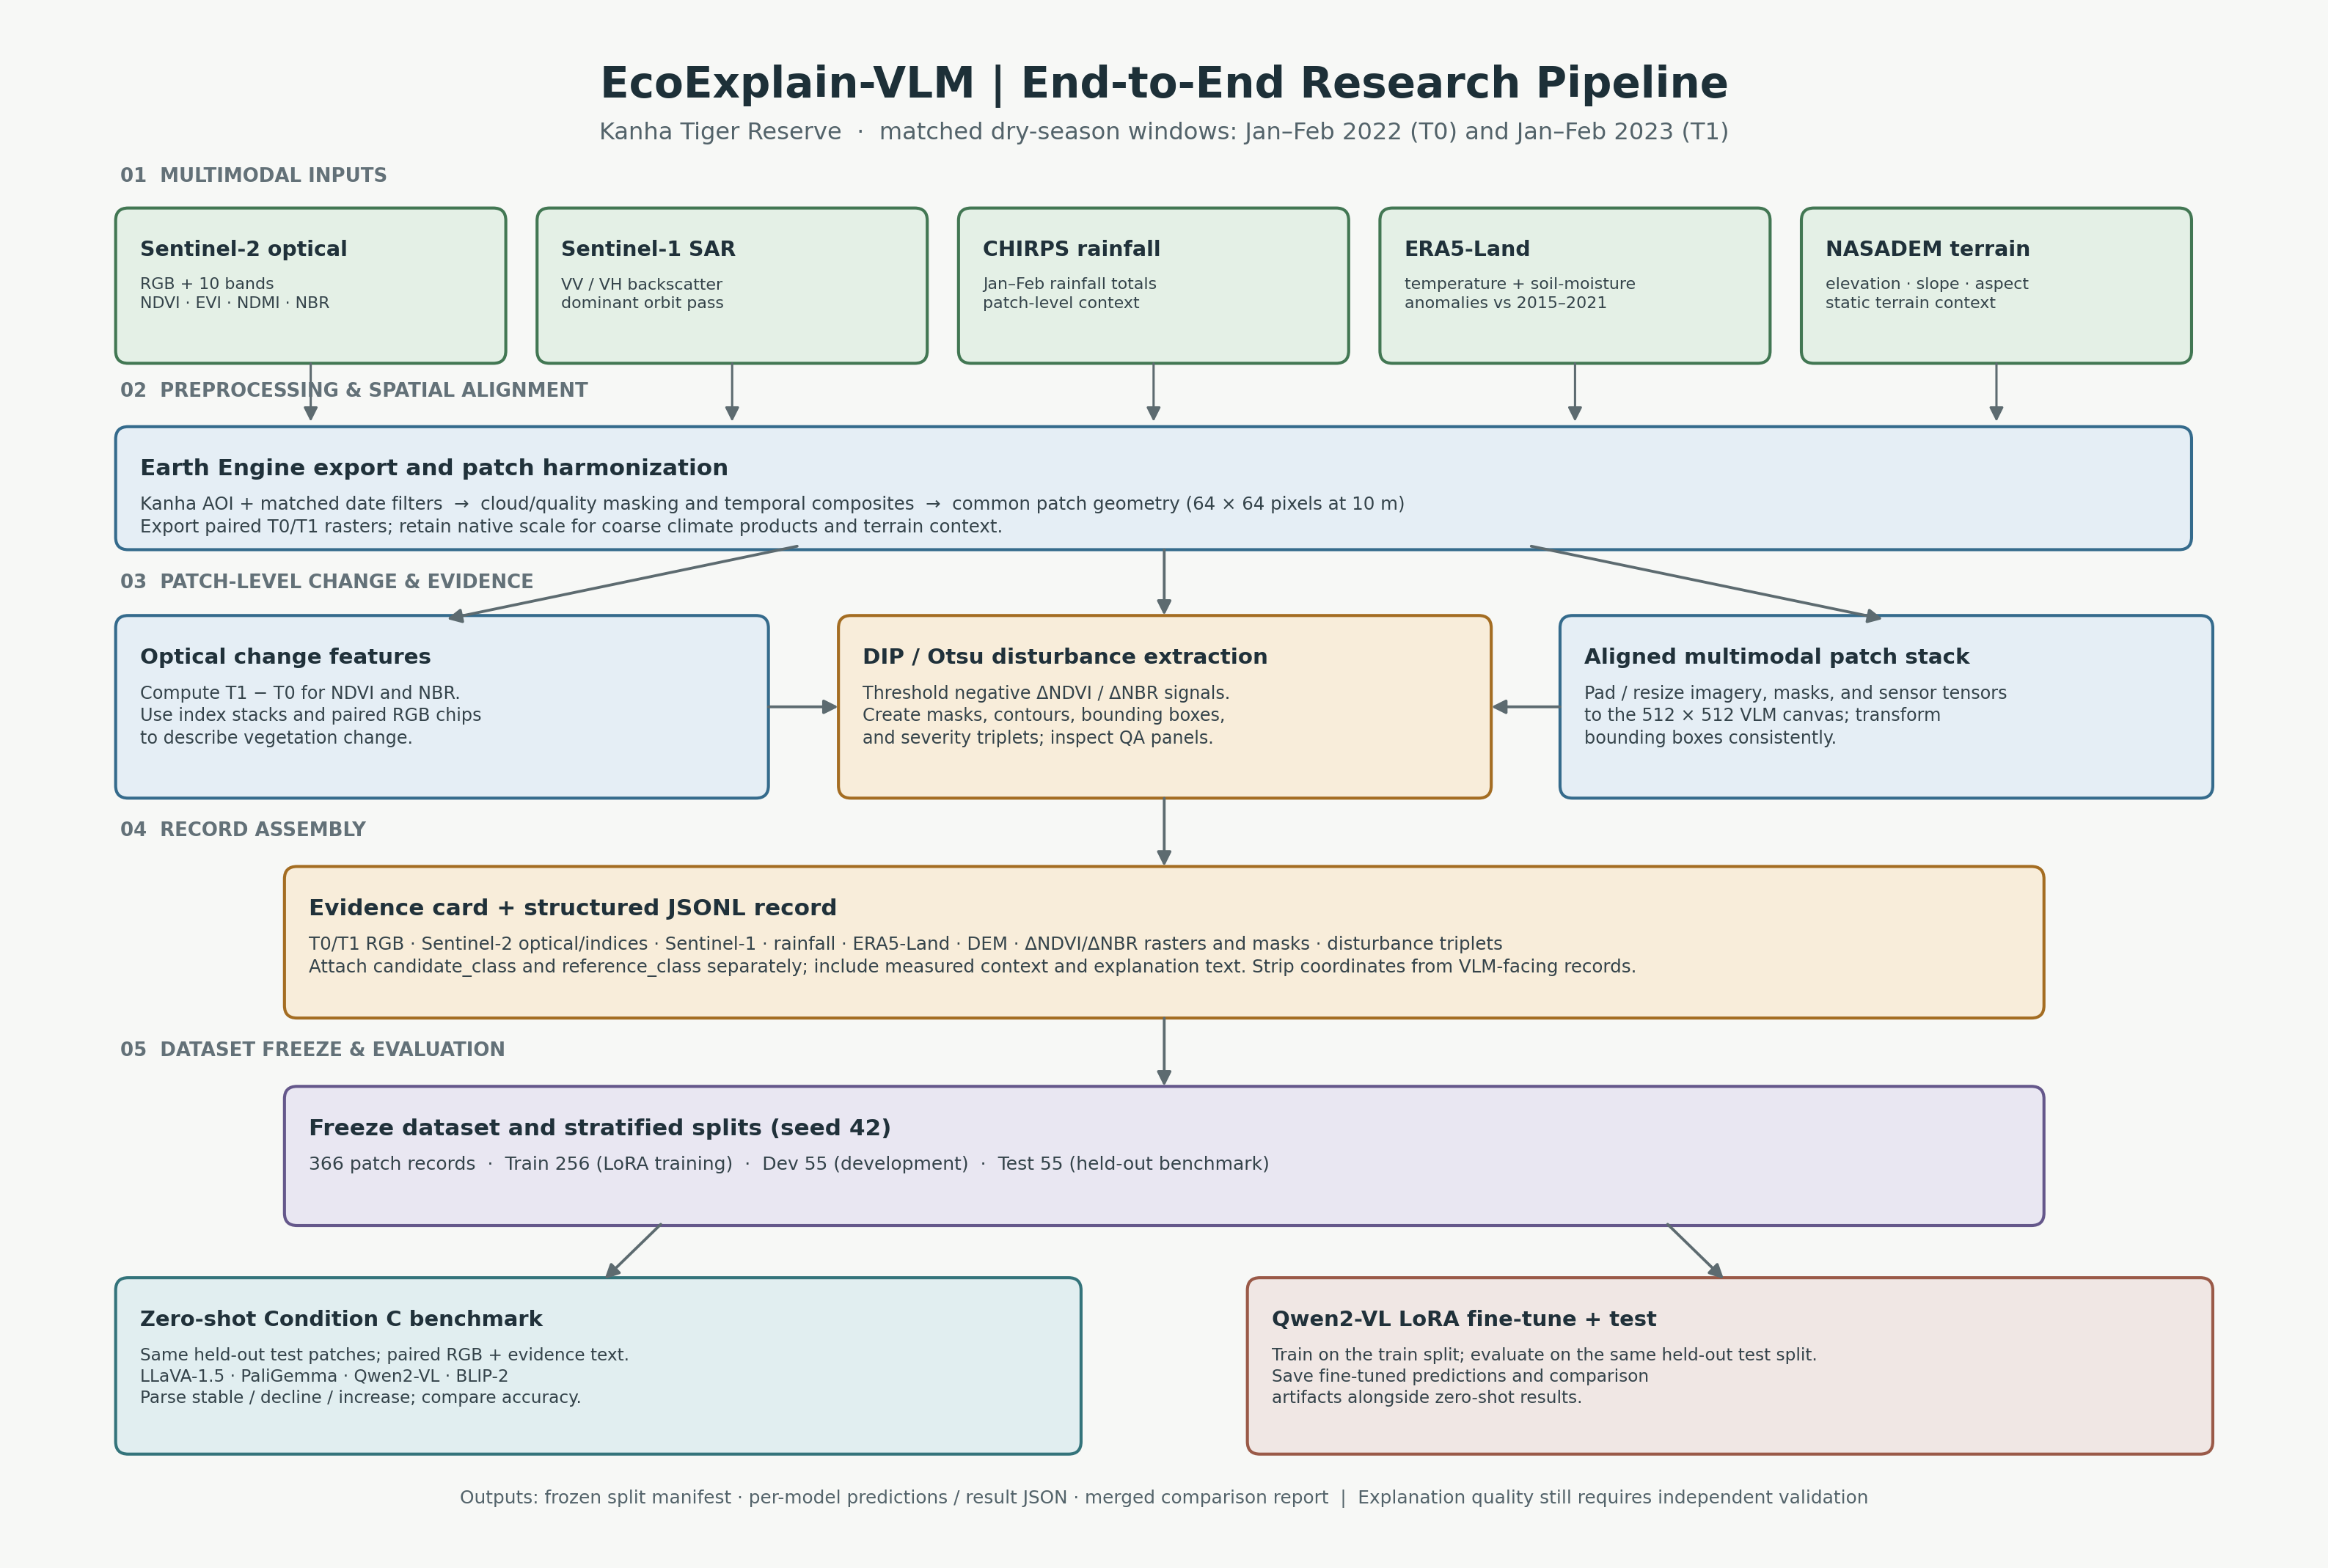
\includegraphics[
    width=\textwidth,
    height=0.78\textheight,
    keepaspectratio
]{results/ecoexplain_vlm_pipeline.png}
\caption{Detailed EcoExplain-VLM workflow, from multimodal geospatial data acquisition and patch processing through evidence-card construction, dataset splitting, and VLM evaluation.}
\label{fig:ecoexplain-vlm-pipeline}
\end{figure}

\section{Data Acquisition and Preprocessing}

\subsection{Acquisition Sources}
The project uses multiple geospatial and environmental sources. These are assembled into a patch-level multimodal dataset.

The major sources are:
\begin{itemize}
    \item Sentinel-2 optical imagery;
    \item Sentinel-1 SAR imagery;
    \item CHIRPS or rainfall data;
    \item ERA5-Land reanalysis product;
    \item DEM or terrain data.
\end{itemize}

\subsection{Preprocessing Stages}
The raw data undergo several preprocessing steps:
\begin{itemize}
    \item AOI clipping;
    \item date filtering;
    \item cloud or quality filtering;
    \item reprojection to a common CRS;
    \item resampling to target resolution;
    \item band selection;
    \item temporal aggregation or compositing;
    \item mask generation;
    \item patch extraction and alignment.
\end{itemize}

\subsection{What Is Verified}
The actual project files indicate that the system creates distinct scene objects containing T0 and T1 data, plus delta masks and evidence outputs. The project explicitly handles:
\begin{itemize}
    \item Landsat-like or Sentinel-like 2-band and 10-band imagery;
    \item delta NDVI and delta NBR generation;
    \item disturbance mask extraction;
    \item VLM input image generation;
    \item structured evidence cards.
\end{itemize}

\subsection{What Is Not Fully Verified}
Some detailed dataset-preprocessing choices may depend on notebook logic or local execution state. In particular:
\begin{itemize}
    \item exact cloud masking policy;
    \item exact resampling kernel choices;
    \item exact aggregation function for multi-scene compositing;
    \item exact handling of nodata or edge artifacts.
\end{itemize}
These preprocessing details should be confirmed against the export notebooks and \texttt{src/gee\_utils.py} when reproducing the pipeline.

\section{Patch Design and Data Representation}

\subsection{Patch Size}
The project uses patch-based processing with dimensions consistent with a $64 \times 64$ pixel grid at approximately 10 m resolution. This yields a physical extent of approximately:
\[
64 \times 10\text{m} = 640\text{m}
\]
in each direction.

\subsection{Why Patches}
Patches are used because:
\begin{itemize}
    \item a local region is more computationally manageable;
    \item local change signals can be interpreted in context;
    \item a VLM can receive a compact image patch;
    \item evidence cards can be assembled around a patch-level disturbance case.
\end{itemize}

\subsection{Patch Alignment}
The project compares T0 and T1 data for the same patch region, ensuring alignment in geospatial coordinates. The data model stores patch-level entries with paired before/after images and associated evidence.

\section{Feature Engineering and Disturbance Detection}

\subsection{Disturbance Logic}
The project uses spectral change features derived from vegetation and burn-related indices. The disturbance logic is built on the difference between T0 and T1 conditions, particularly:
\begin{itemize}
    \item delta NDVI;
    \item delta NBR.
\end{itemize}

The core logic checks for decreases in vegetation signal or burn-sensitive change patterns, then extracts spatial bounding boxes around the affected pixels.

\subsection{Otsu-Based Thresholding}
The implementation uses Otsu thresholding to identify informative change regions in the spectral difference maps. This is a standard approach for separating foreground disturbance regions from background signal.

The project logic in its source utilities explicitly describes:
\begin{itemize}
    \item disturbance detection from spectral drops;
    \item extraction of bounding boxes around changed pixels;
    \item severity classification by mean drop magnitude;
    \item merging of overlapping boxes;
    \item choosing the most relevant disturbance boxes for each patch.
\end{itemize}

\section{Dataset Construction}

\subsection{Evidence Cards}
The final dataset is a JSONL-based record set where each row corresponds to a patch. Each record includes:
\begin{itemize}
    \item scene ID;
    \item time-pair images;
    \item sensor-specific arrays and metadata;
    \item indices and masks;
    \item disturbance triplets;
    \item candidate label;
    \item reference label if available;
    \item explanation text;
    \item source metadata.
\end{itemize}

\subsection{Label Types}
The project distinguishes between:
\begin{itemize}
    \item \textbf{candidate\_class}: a class assigned using the project’s automatic change logic or model-based inference;
    \item \textbf{reference\_class}: a human or curated label when available.
\end{itemize}

This distinction is important because many of the code paths explicitly accommodate both generated labels and human labels.

\subsection{Final Dataset Size}
The project’s concrete dataset artifact contains 366 rows. This is a verified output from the project files.

\subsection{Train/Dev/Test Split}
Splits were frozen with seed 42 and stratification on \texttt{candidate\_class}: train 256, development 55, test 55 patches. All benchmark accuracies in this report use the test split only. Manifest: \texttt{data/splits/split\_manifest.json}.

\section{Modeling and Architecture}

\subsection{Vision-Language Model Fundamentals}
A vision-language model combines:
\begin{itemize}
    \item a vision encoder that transforms image inputs into visual representations;
    \item a language model that processes text and produces token-level outputs;
    \item a multimodal alignment or projection mechanism that connects image features to the language space.
\end{itemize}

The benefit is that image evidence and text prompts can be jointly processed. This is useful in geospatial analysis because prompts can specify classes, include evidence descriptions, or ask for structured outputs.

\subsection{Project-Specific Use of VLMs}
The project evaluates several VLM families:
\begin{itemize}
    \item Qwen2-VL;
    \item PaliGemma;
    \item LLaVA-NeXT-Interleave 0.5B (\texttt{llava-interleave-qwen-0.5b-hf});
    \item BLIP-2 OPT-2.7B.
\end{itemize}

\subsection{Condition C Protocol}
\textbf{Condition~C} denotes combined inputs: paired T0/T1 RGB chips plus the multimodal evidence narrative stored in each JSONL record (indices, SAR, rainfall, temperature and soil-moisture anomalies, terrain, and data-quality notes). Qwen and LLaVA received the full card (truncated for context limits); PaliGemma and BLIP-2 used shorter text prompts in the zero-shot notebooks, as documented in the evaluation code. The card ends with the pipeline's rule-based summary line (\texttt{vegetation\_trend=\dots, candidate\_class=\dots}), and \texttt{candidate\_class} is also the field used as the evaluation label; Condition~C accuracy therefore measures how well a model uses the complete evidence card. A sensitivity variant with this line removed (\texttt{evidence\_only}) is reported in Section~\ref{sec:sensitivity}.

The benchmark uses structured label extraction from generated text, where the model is asked to produce a class such as:
\begin{itemize}
    \item stable;
    \item decline;
    \item increase.
\end{itemize}

The result is parsed from model output to evaluate classification accuracy.

\subsection{Zero-Shot Evaluation}
Zero-shot evaluation means the model is used without task-specific fine-tuning on the target dataset. The project benchmark uses the same test split across models and compares the parsed class output against the class target.

\subsection{Fine-Tuning}
The project includes a LoRA fine-tuning workflow for Qwen2-VL (\texttt{src/vlm\_finetune.py}, \texttt{scripts/run\_finetune\_qwen.py}, notebook 09, Ada Slurm). The headline fine-tuned result (\textbf{67.3\,\%} test accuracy) comes from Ada job 2722446: smoke configuration with 16 training patches, one epoch, 4-bit quantised LoRA ($r=8$), evaluated on the same 55 test patches under Condition~C. Full training-split runs and merged adapters are documented in cluster logs under \texttt{ada\_review/}.

\begin{table}[H]
\centering
\renewcommand{\arraystretch}{1.2}
\begin{tabular}{p{4cm} p{9cm}}
\toprule
\textbf{Model / Setup} & \textbf{Status} \\
\midrule
Zero-shot Qwen2-VL & Implemented and benchmarked \\
Zero-shot PaliGemma & Implemented and benchmarked \\
Zero-shot LLaVA-Interleave 0.5B & Implemented and benchmarked \\
Zero-shot BLIP-2 & Implemented and benchmarked \\
Qwen2-VL LoRA fine-tune & Implemented and evaluated \\
\bottomrule
\end{tabular}
\caption{Model implementations present in the project.}
\end{table}

\section{Explainability and Explanation Evaluation}

\subsection{Motivation}
After establishing Condition~C classification benchmarks (including \textbf{67.3\,\%} for fine-tuned Qwen), the study prioritised whether models can \textbf{justify} their decisions in language aligned with the evidence table---not only whether they predict \texttt{stable}, \texttt{decline}, or \texttt{increase}.

\subsection{Explanation Mode (Implemented)}
\texttt{scripts/run\_explain.py} prompts each VLM with a compact numeric evidence table (\texttt{src/vlm\_evidence.py}) and requests a class plus justification (JSON for Qwen/LLaVA; shortened prompts for PaliGemma/BLIP-2). Outputs are stored under \texttt{results/explain/explain\_*.json}. \texttt{scripts/score\_explanations.py} and \texttt{src/explain\_metrics.py} extract checkable claims (e.g.\ rainfall, NDVI direction) and compare them to the evidence.

\subsection{Structured Cite-Only Protocol}
The first (legacy) explanation prompt left models free to describe and speculate. A structured variant (\texttt{--prompt-style structured}) was therefore added. Each prompt contains the compact evidence table, a numbered list of \texttt{ALLOWED\_FACTS} built from the record (NDVI in both years, EVI and NDMI change, rainfall, temperature anomaly, VV change), and a \texttt{CLASS\_RULE} line stating the NDVI rule for that patch with $\pm0.02$ cut-offs (\texttt{compact\_evidence\_structured} in \texttt{src/vlm\_evidence.py}). The instruction (\texttt{EXPLAIN\_JSON\_ASK\_STRUCTURED}) asks the model to copy three facts verbatim, set the class using the rule, write one sentence about NDVI only, and state no climate causes. Outputs are written to \texttt{results/explain/explain\_structured\_*.json}. Qwen2-VL-2B and LLaVA-Interleave-0.5B were run on all 55 test patches on a MacBook Air using the Apple GPU (MPS) on 6 October 2026 (1,009\,s and 414\,s respectively; greedy decoding, up to 256 new tokens). An Ada job for the same protocol was prepared but the reported results come from the local runs.

\subsection{Automatic Metrics}
Per-model aggregates are in \texttt{results/explain/explanation\_scores.csv} (one row per model, structured run preferred):
\begin{itemize}
    \item \textbf{Classification accuracy} from explain-mode parsing (may differ from one-word Condition~C runs).
    \item \textbf{Fraction of correct checkable claims} among extracted statements.
    \item \textbf{Hallucination / inconsistency flags}, ROUGE-L overlap with evidence vs.\ template text, and \textbf{distinct-2} diversity (repetition).
\end{itemize}
These metrics measure \emph{evidence consistency}, not human plausibility; they are appropriate for a pilot automatic audit. A claim is counted as correct when its direction matches the measured change, with changes below a dead-band (0.02 for indices, 0.05 for RGB green cover) treated as stable. Self-consistency excludes explanations in which two claimed directions are equally frequent.

\section{Evaluation and Metrics}

\subsection{Classification Metrics}
The project’s benchmark uses classification accuracy as the primary metric. Accuracy is computed by comparing the model’s parsed output against the target class.

\[
\text{Accuracy} = \frac{\text{Correct predictions}}{\text{Total predictions}}
\]

This is the metric most directly available in the benchmark output.

\subsection{Other Metrics}
Other metrics may be relevant in principle, but they are not clearly verified as the primary project metrics in the final outputs. Metrics such as precision, recall, F1, and confusion matrices are not always clearly reported in the project artifacts.

Macro-F1 and Wilson confidence intervals can be computed from saved per-patch predictions; the repository JSONs report accuracy as the primary classification metric.

\section{Experiments and Results}

\subsection{Dataset Split Design}
The project describes a stratified split with train/dev/test partitions. The actual implementation is based on the project’s split-generation script and data artifact.

\subsection{Zero-Shot Results}
The project contains a benchmark table ranking multiple VLMs.

\begin{table}[H]
\centering
\renewcommand{\arraystretch}{1.2}
\begin{tabular}{p{2cm} p{4cm} p{3cm} p{2.2cm}}
\toprule
\textbf{Rank} & \textbf{Model} & \textbf{Status} & \textbf{Accuracy} \\
\midrule
1 & Qwen2-VL & Zero-shot & 56.4\% \\
2 & PaliGemma & Zero-shot & 36.4\% \\
3 & LLaVA-Interleave 0.5B & Zero-shot & 32.7\% \\
4 & BLIP-2 & Zero-shot & 32.7\% \\
\bottomrule
\end{tabular}
\caption{Verified zero-shot VLM benchmark results.}
\end{table}

\subsection{Fine-Tuned Results}
The project’s fine-tuned Qwen model reports improved test performance.

\begin{table}[H]
\centering
\renewcommand{\arraystretch}{1.2}
\begin{tabular}{p{4cm} p{4cm} p{2.5cm}}
\toprule
\textbf{Model} & \textbf{Setup} & \textbf{Accuracy} \\
\midrule
Qwen2-VL & Zero-shot & 56.4\% \\
Qwen2-VL (fine-tuned) & LoRA fine-tune & 67.3\% \\
\bottomrule
\end{tabular}
\caption{Fine-tuned benchmark uplift (Qwen2-VL-2B, LoRA smoke run on Ada).}
\end{table}

\begin{figure}[H]
\centering
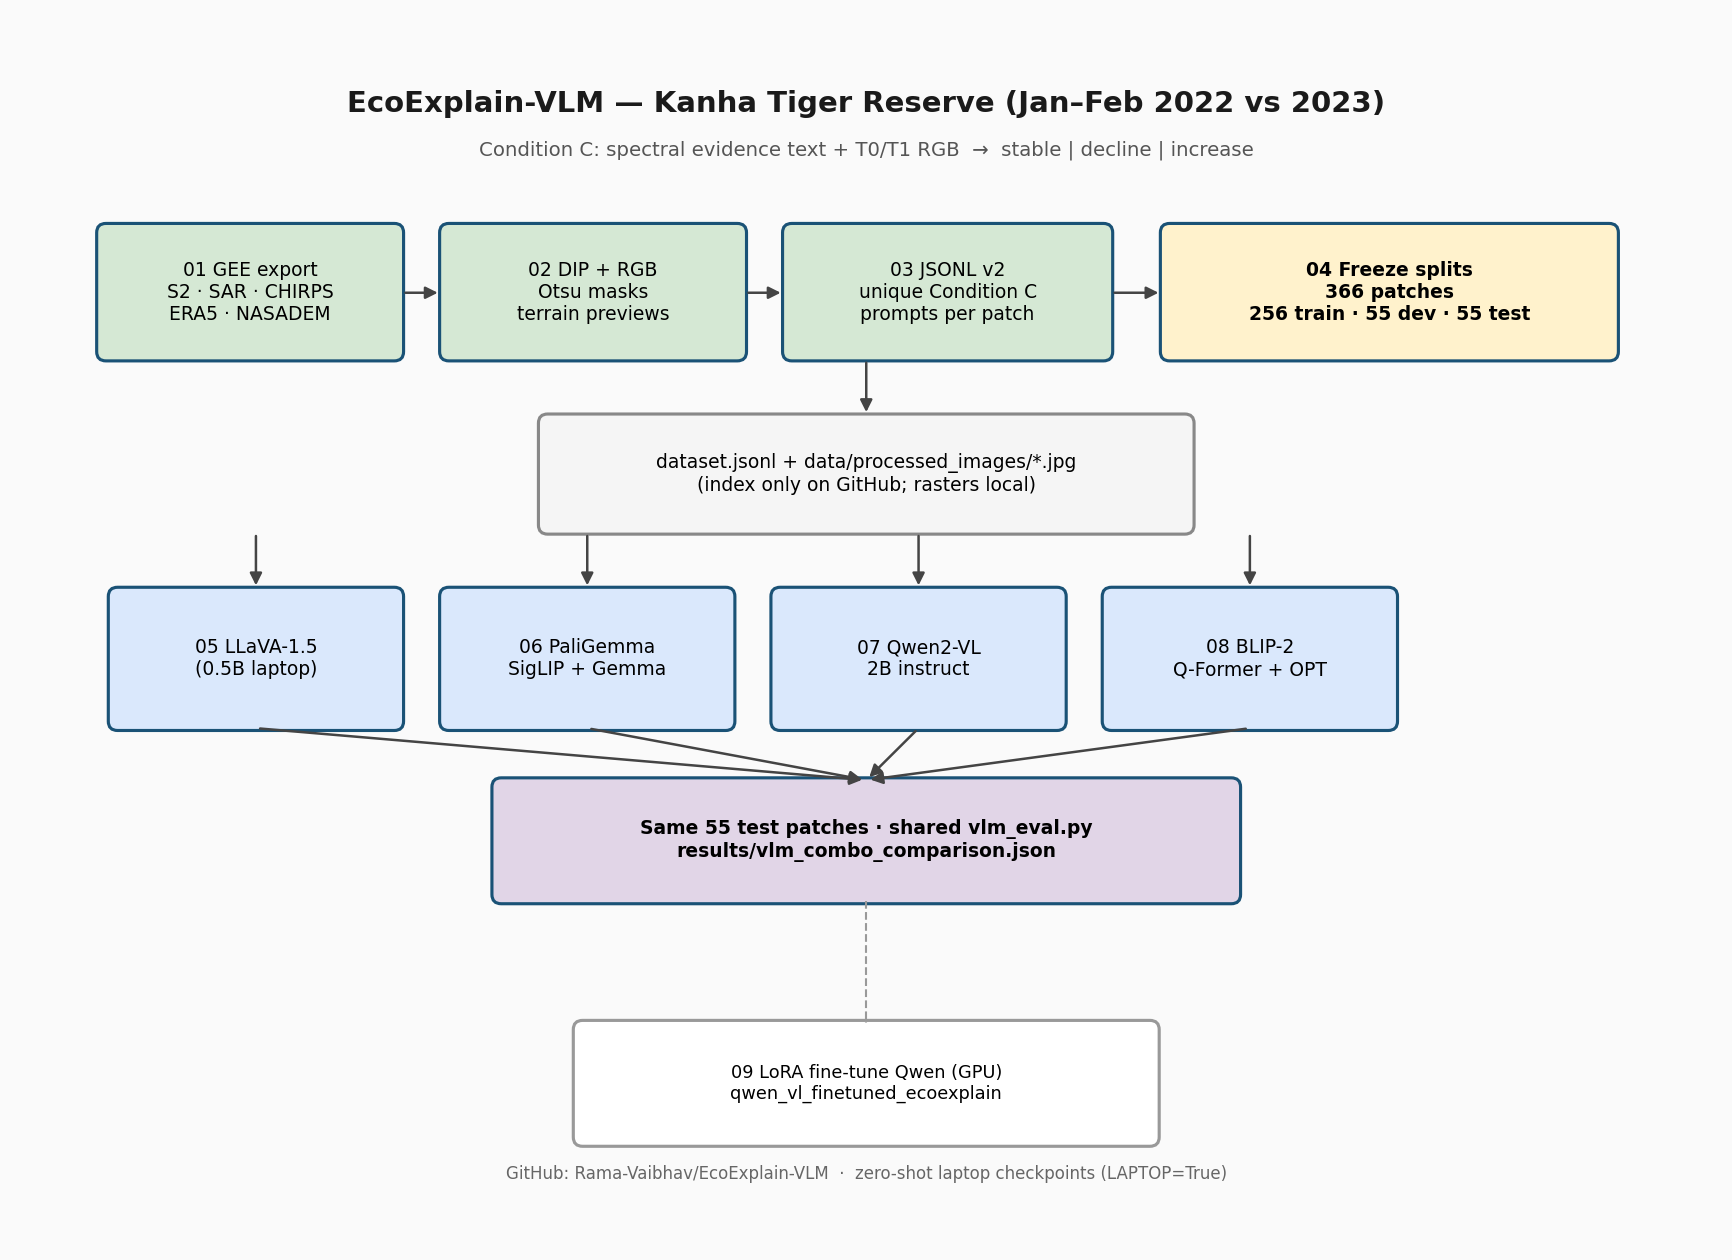
\includegraphics[width=0.95\textwidth]{results/result1.png}
\caption{Pipeline overview figure (\texttt{results/result1.png}).}
\label{fig:result1}
\end{figure}

\begin{figure}[H]
\centering
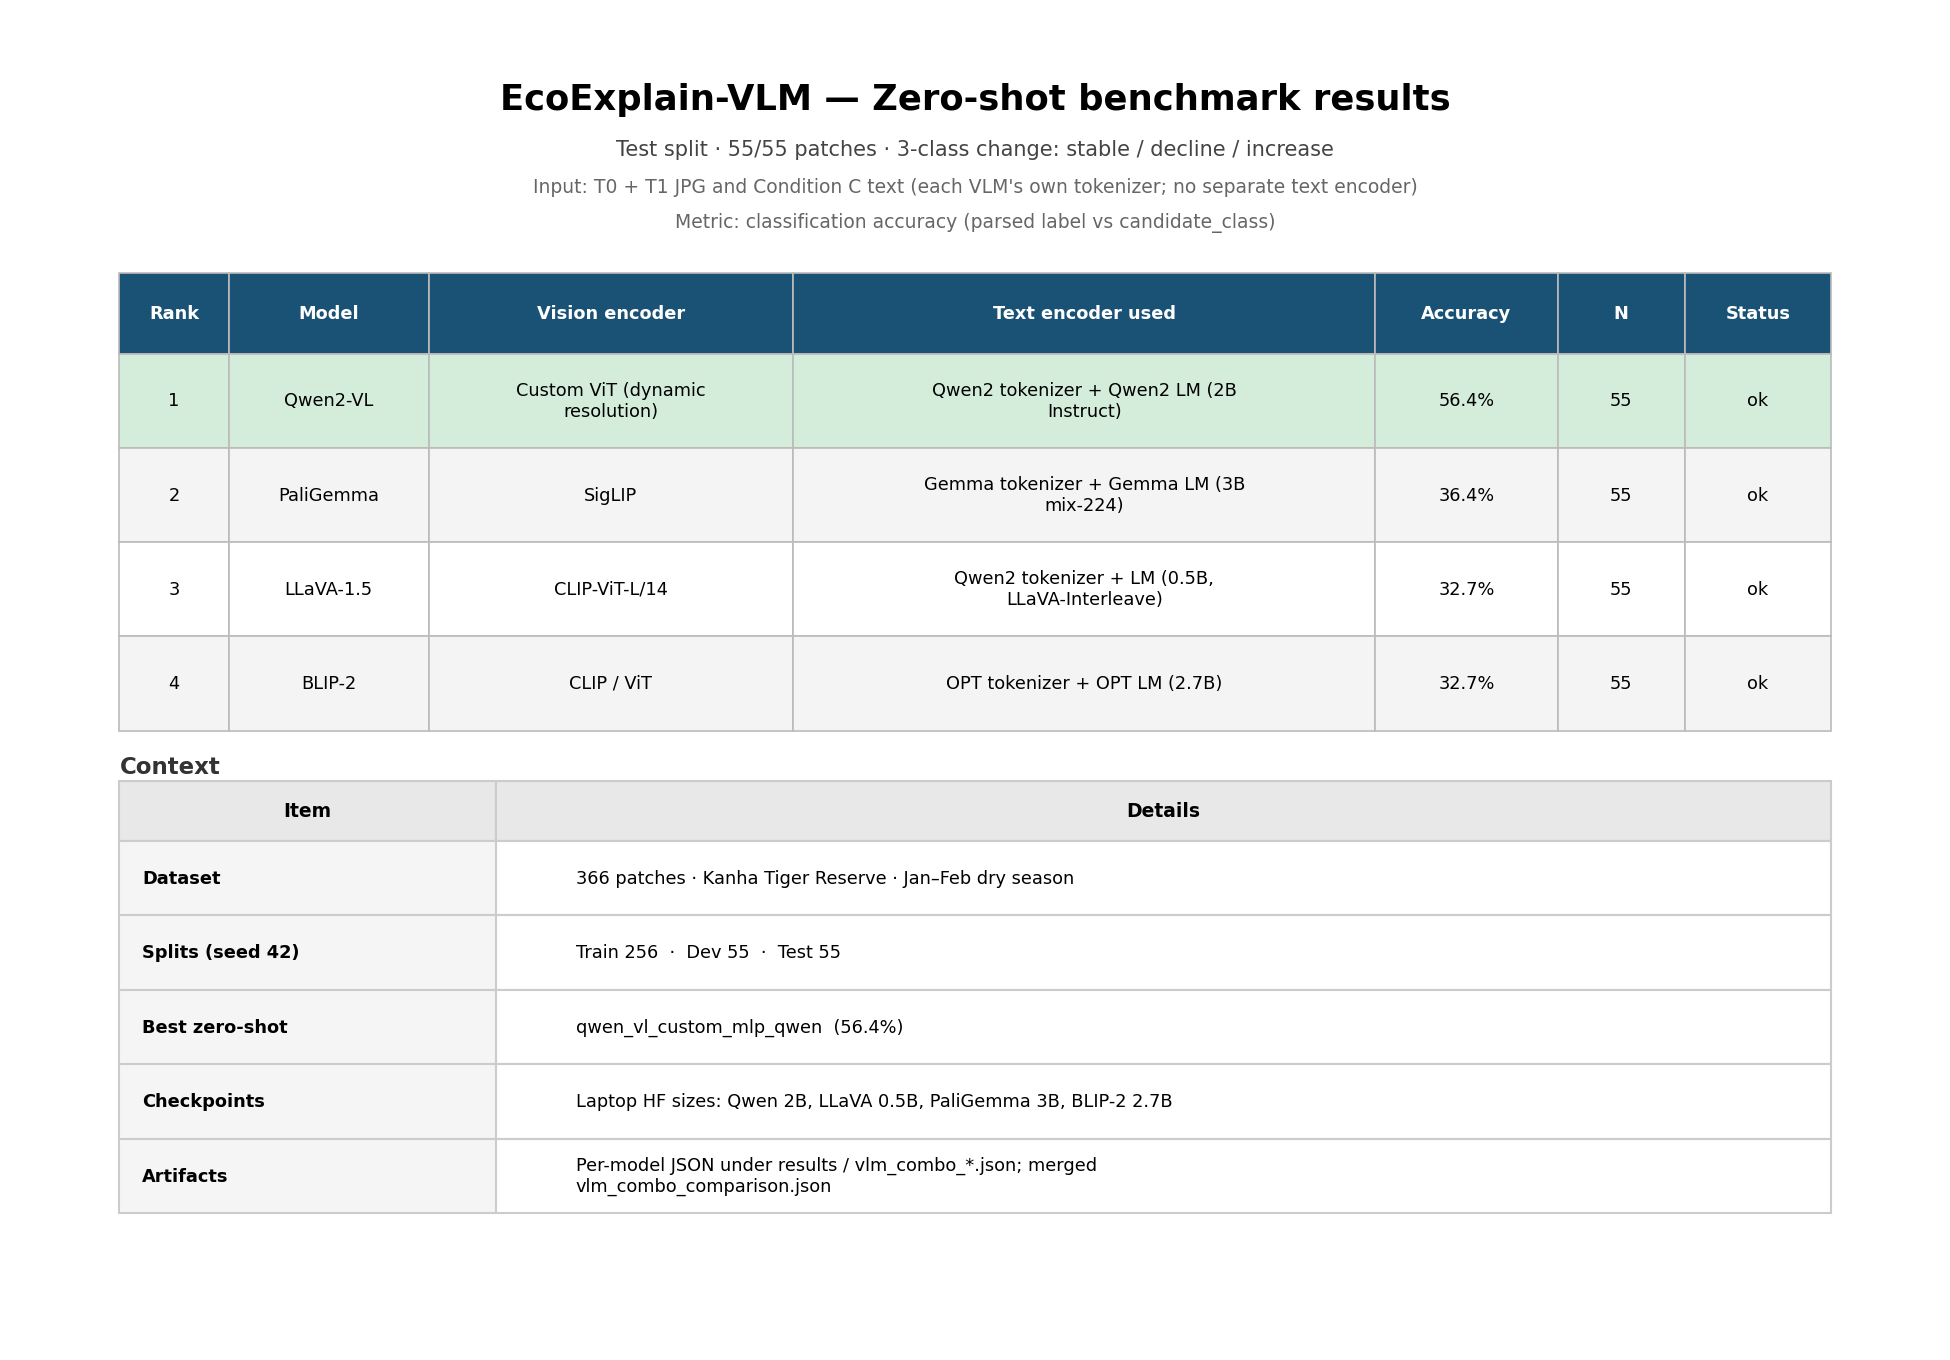
\includegraphics[width=0.95\textwidth]{results/result2.png}
\caption{Zero-shot model comparison on the test split (\texttt{results/result2.png}).}
\label{fig:result2}
\end{figure}

\subsection{Explanation-Mode Results}

Table~\ref{tab:explain-structured} gives the structured-protocol results; Table~\ref{tab:explain-scores} gives the earlier free-form (legacy) results for comparison.

\begin{table}[H]
\centering
\renewcommand{\arraystretch}{1.2}
\begin{tabular}{p{6.2cm} r r}
\toprule
 & \textbf{Qwen2-VL-2B} & \textbf{LLaVA-Interleave 0.5B} \\
\midrule
Explain-mode class accuracy & 63.6\% (35/55) & 45.1\% (23/51) \\
Class agrees with stated \texttt{CLASS\_RULE} & 53/55 & 42/55 \\
Checkable claims per explanation & 2.85 & 2.33 \\
Correct claims & 75.8\% & 71.1\% \\
Explanations with $\geq$1 flagged claim & 36.4\% & 34.5\% \\
Self-consistency & 100\% & 90.7\% \\
ROUGE-L vs.\ evidence table & 0.566 & 0.250 \\
\bottomrule
\end{tabular}
\caption{Structured cite-only explanations on the test split ($n=55$), MacBook Air (MPS), October 2026. Source: \texttt{results/explain/explanation\_scores.csv}.}
\label{tab:explain-structured}
\end{table}

\begin{table}[H]
\centering
\renewcommand{\arraystretch}{1.2}
\begin{tabular}{p{3.8cm} r r r r}
\toprule
\textbf{Model} & \textbf{Explain acc.} & \textbf{Claims / expl.} & \textbf{\% correct claims} & \textbf{Near-dup. share} \\
\midrule
Qwen2-VL-2B & 3/3 ($n=3$) & 5.33 & 43.8\% & 0 \\
LLaVA-Interleave 0.5B & 29.1\% & 1.09 & 56.7\% & 34.5\% \\
PaliGemma-3B & 33.3\% (of 36) & 0 & --- & 100\% \\
BLIP-2 OPT-2.7B & 32.7\% & 0 & --- & 100\% \\
\bottomrule
\end{tabular}
\caption{Legacy (free-form) explanation prompt (\texttt{score\_explanations.py --include-legacy}). Qwen was run on three test patches with this prompt.}
\label{tab:explain-scores}
\end{table}

\subsection{Interpretation}
\textbf{Classification.} Qwen2-VL-2B is the only model clearly above the others under Condition~C; LoRA adaptation yields an \textbf{11-point} absolute gain on the same test split (56.4\,\% $\rightarrow$ 67.3\,\%). Because the Condition~C card includes the pipeline's summary line, these figures describe use of the complete card. Results are specific to Kanha, the Jan--Feb 2022/2023 pair, percentile-based labels, and the open-model scale used.

\textbf{Explanations.} With the free-form prompt, justifications were missing, repetitive, or factually inconsistent with the evidence table (for example, attributing change to increased rainfall when rainfall fell). The structured cite-only prompt raised the share of correct claims to 75.8\,\% (Qwen) and 71.1\,\% (LLaVA). Of the claims still flagged, 35 of 38 (Qwen) and 35 of 37 (LLaVA) describe a true change smaller than the scoring dead-band; only one Qwen claim and two LLaVA claims state the wrong direction. The trade-off is that the class follows the stated rule (Qwen agreed with \texttt{CLASS\_RULE} on 53 of 55 patches, which is why its explain-mode accuracy equals the rule's 63.6\,\%) and justifications largely restate supplied facts (ROUGE-L 0.566 against the evidence table for Qwen).

\subsection{Sensitivity Analyses}
\label{sec:sensitivity}
With the summary line removed (\texttt{evidence\_only}), PaliGemma, LLaVA and BLIP-2 scored 36.4\,\%, 36.4\,\% and 32.7\,\% on the 55 test patches (\texttt{results/explain/oneword\_*.json}); Qwen was run on three patches in this mode. A two-threshold rule on the card's $\Delta$NDVI value reaches 94.5\,\% (thresholds fitted on the training split). Longer LoRA runs with the full card (Ada jobs 2690 and 2792) reached 100\,\% test accuracy, indicating that the fine-tuned model can learn to read the summary line.

\section{Traceability Matrix}

The following matrix maps major research claims to the implementation evidence level.

\begin{table}[H]
\centering
\renewcommand{\arraystretch}{1.25}
\small
\begin{tabular}{p{3.5cm} p{3cm} p{3.2cm} p{3.6cm} p{2.3cm}}
\toprule
\textbf{Research claim} & \textbf{Planned method} & \textbf{Actual code} & \textbf{Evidence} & \textbf{Status} \\
\midrule
Forest disturbance monitoring & Remote sensing and patch classification & Implemented geospatial pipeline & Data files, scripts, outputs & Implemented \\
Multi-source data integration & Optical + SAR + climate + terrain & Present in code and data records & Evidence cards and source modules & Implemented \\
Patch-based classification & Local image patches & Implemented with 64x64 style patch design & Dataset, configuration, code & Implemented \\
DIP / Otsu disturbance extraction & Spectral difference masks & Present in source utilities & Disturbance triplets and masks & Implemented \\
Zero-shot VLM benchmark & Compare models on the same test set & Implemented in evaluation code & Result JSON files & Implemented \\
Fine-tuning pipeline & LoRA training for Qwen & Implemented & Fine-tune script and result artifact & Implemented \\
Explainable reasoning & Grounded narrative and evidence & \texttt{run\_explain.py}, scoring pipeline & \texttt{results/explain/} & Implemented \\
Formal XAI validation & Human faithfulness / causal tests & Automatic claim metrics only & \texttt{explanation\_scores.csv} & Partial (pilot) \\
Full scientific validation & Benchmarked across many regions & Pilot-scale dataset and setup & Project artifact set & Partial \\
\bottomrule
\end{tabular}
\caption{Traceability matrix linking research aims to actual implementation evidence.}
\end{table}

\section{Limitations and Weaknesses}

\subsection{Data Limitations}
\begin{itemize}
    \item The project uses a limited geographic pilot area.
    \item Temporal coverage is narrow and compared only across two dry-season periods.
    \item A single-ROI setup limits generalization.
    \item Sensor availability and pre-processing assumptions may affect comparability.
\end{itemize}

\subsection{Label Limitations}
\begin{itemize}
    \item Candidate and reference labels are not always equivalent.
    \item The project explicitly distinguishes between generated class logic and human reference labels.
    \item Evaluation is therefore strong for project-specific benchmark design but not necessarily for universal ecological truth.
\end{itemize}

\subsection{Methodological Limitations}
\begin{itemize}
    \item Labels follow automatic percentile rules on $\Delta$NDVI with only 19 human reference checks in the pilot set.
    \item The split is random-stratified, not spatially blocked; test size is 55 patches (wide confidence intervals).
    \item Explanation metrics are regex-based evidence-consistency checks, not blind human ratings.
    \item Zero-shot models did not all receive identical text length (Qwen/LLaVA full card vs.\ shorter prompts for PaliGemma/BLIP-2).
    \item LoRA headline used a 16-patch smoke train; full 256-patch training logs exist separately on Ada.
    \item The Condition~C card includes the pipeline's summary line with \texttt{candidate\_class}; the \texttt{evidence\_only} sensitivity run covers three models on all 55 patches and Qwen on three.
    \item Structured explanations were run for Qwen and LLaVA only; most outputs exceeded the 256-token limit before closing the JSON, and the class follows the stated NDVI rule.
\end{itemize}

\subsection{Computational Limitations}
\begin{itemize}
    \item Model inference and fine-tuning require substantial compute.
    \item Large geospatial datasets can be heavy to store and process.
    \item Reproducible full-scale training may require GPU infrastructure.
\end{itemize}

\section{Future Work}
\subsection{Label epistemology and spatial validation}
Progress from distribution-derived operational labels to dual independent expert interpretation with inter-rater reliability; adopt spatial block cross-validation so map-level performance accounts for autocorrelation among neighbouring patches.

\subsection{Modality and representation}
Systematic Conditions A--B (vision-only vs.\ tabular-only) ablations; RS-tuned VLMs and false-colour / change-index inputs to study domain shift from natural-image pre-training.

\subsection{Probabilistic and human-centred explanation science}
Calibrated confidence (Brier score, expected calibration error); blind human faithfulness ratings; counterfactual evidence edits; teacher--student distillation of consistent justifications (\texttt{build\_explain\_targets.py}).

\subsection{Spatio-temporal generalisation}
Multi-year stacks and additional central-Indian reserves (e.g.\ Pench, Achanakmar) to separate drought, phenology, and structural disturbance; fusion of active-fire layers for richer disturbance typing.

\section{Reproducibility and Practical Usage}

\subsection{Environment}
The project uses a Python environment with geospatial, ML, and remote-sensing dependencies. This is implemented in a project virtual environment and is suitable for notebook and script execution.

\subsection{Typical Workflow}
\begin{enumerate}
    \item prepare the environment;
    \item acquire or locate raw geospatial files;
    \item export scenes and build patch datasets;
    \item generate spectral indices and masks;
    \item construct evidence-card records;
    \item run VLM benchmark;
    \item run fine-tuning if required;
    \item evaluate accuracy and inspect explanations.
\end{enumerate}

\section{Glossary}
\begin{description}[leftmargin=1.5em]
    \item[AOI] Area of Interest.
    \item[SAR] Synthetic Aperture Radar.
    \item[Sentinel-1] Copernicus SAR mission.
    \item[Sentinel-2] Copernicus optical mission with MSI.
    \item[MSI] Multispectral Instrument.
    \item[VV] Vertical transmit, vertical receive polarization.
    \item[VH] Vertical transmit, horizontal receive polarization.
    \item[Backscatter] Radar signal returned to the sensor.
    \item[Speckle] Radar image noise from interference.
    \item[NDVI] Normalized Difference Vegetation Index.
    \item[NDMI] Normalized Difference Moisture Index.
    \item[NBR] Normalized Burn Ratio.
    \item[EVI] Enhanced Vegetation Index.
    \item[DEM] Digital Elevation Model.
    \item[CRS] Coordinate Reference System.
    \item[Raster] Grid-based spatial data.
    \item[Pixel] Smallest unit of a raster image.
    \item[Patch] Local spatial region used as a model input.
    \item[VLM] Vision-Language Model.
    \item[Explainability] Ability to provide interpretable reasoning for predictions.
    \item[Fine-tuning] Updating model weights on task-specific data.
    \item[Inference] Applying the trained model to new inputs.
    \item[Operational label] \texttt{candidate\_class} used for benchmark accuracy (automatic rule-based).
\end{description}

\section{Conclusion}
EcoExplain-VLM delivered a reproducible five-source Kanha benchmark (366 patches, frozen splits) and a controlled open-VLM evaluation under Condition~C. \textbf{Qwen2-VL-2B} achieved \textbf{56.4\,\%} zero-shot test accuracy and \textbf{67.3\,\%} after LoRA fine-tuning, clearly ahead of the other models tested, under the project's Condition~C protocol, in which the evidence card includes the pipeline's own summary line.

The study then showed that \textbf{classification success does not imply trustworthy explanations}: with a free-form prompt, automatic scoring found missing, repetitive, or evidence-inconsistent justifications across architectures. A structured cite-only prompt raised claim correctness to 75.8\,\% (Qwen2-VL-2B) and 71.1\,\% (LLaVA-Interleave-0.5B) on the full test set, with very few claims of the wrong direction, at the cost of explanations that mostly restate supplied facts. That contrast between free and constrained explanation is the central interpretive contribution.

Together, the dataset, code, benchmark JSONs, explanation artifacts, and Ada fine-tuning workflow form a completed Independent Study suitable for extension via spatial validation, human explanation rating, and larger or RS-specialised models. Claims should remain scoped to Kanha, the 2022--2023 dry-season window, and the automatic label design described above.

\end{document}
